\section{CU1 - Diagramme général}

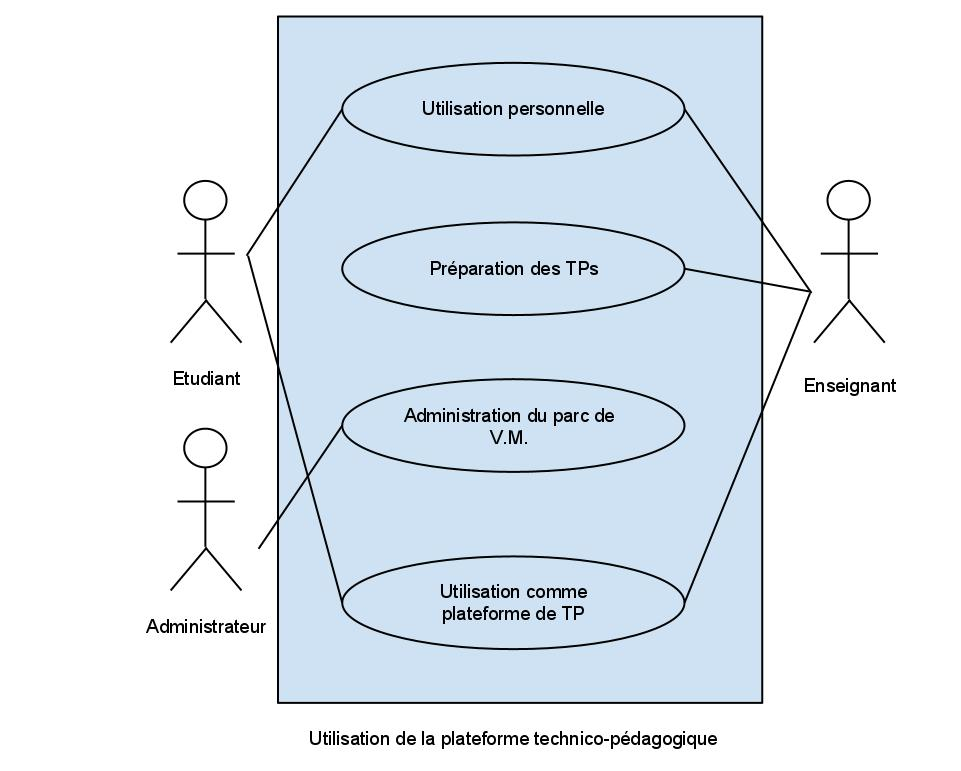
\includegraphics[scale=0.4]{CU1.jpg}

Dans l’organisation générale de cet outil pédagogique, nous pouvons identifier différents acteurs. Il y a tout d’abord l’étudiant, au coeur du système : il a la possibilité de s’identifier et d’utiliser les Machines Virtuelles mises à sa disposition. L’enseignant possède dans cet outil les mêmes cas d’utilisation de base que les étudiant. Il peut en outre utiliser la plate-forme mise à sa disposition pour préparer des travaux pratiques spécifiques et fournir des machines virtuelles de travail aux étudiants. Enfin, le dernier acteur utilisant ce produit est l’administrateur : Il a la possibilité d’administrer le parc de machines virtuelles.
